\documentclass[../main.tex]{subfiles}

\begin{document}

\subsubsection*{Methodology}
\subsubsection*{Data analysis}

    \begin{figure}[H]
        \centering
        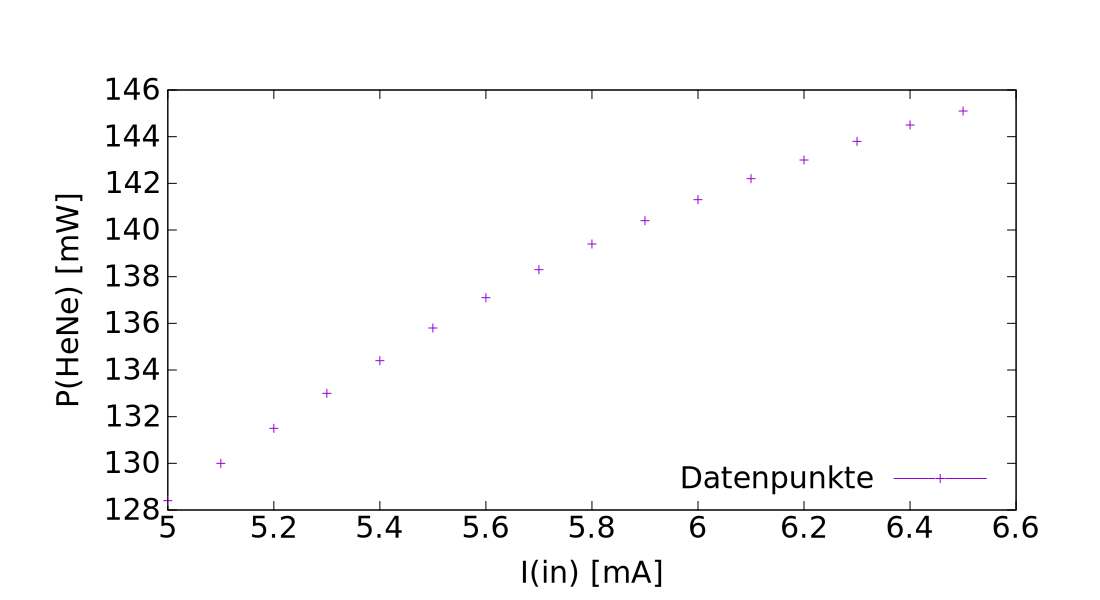
\includegraphics[width=0.8\textwidth]{Bilddateien/6/P(HeNe)overI(in).png}
        \caption{Output power as a function of the input power with the $850\;\si{\mm}$ curved mirror.}
        \label{fig:output_power_over_input_power_curved}
    \end{figure}

    This time we can clearly see a concave nature of the dependency, but we assume the last points to be nearly at the same amplitude which would indicate a saturation in the higher current range. 

    Lastly we observed two modes in the resonator of the HeNe laser. They are displayed in figure \ref{fig:TEM_0_1} and \ref{fig:TEM_1_0}.
    \begin{figure}[H]
        \centering
        \begin{subfigure}[b]{0.4\textwidth}
            \centering
            \includegraphics[angle=0,width=\textwidth]{Bilddateien/6/IMG_3497.jpeg}
            \caption{$\text{TEM}_{0,1}$}
            \label{fig:TEM_0_1}
        \end{subfigure}
        \begin{subfigure}[b]{0.4\textwidth}
            \centering
            \includegraphics[angle=180,width=\textwidth]{Bilddateien/6/IMG_3499.jpeg}
            \caption{$\text{TEM}_{1,0}$}
            \label{fig:TEM_1_0}
        \end{subfigure}
        \caption{The two captured modes of the HeNe laser given in \emph{rectangular transverse modes}.}
    \end{figure}
    For classification we use the \emph{transverse electromagnetic modes} model, short \emph{TEM}. The first number indicates the number of nodes in the $x$ direction and the second number the number of nodes in the $y$ direction. The mode $\text{TEM}_{0,1}$ is therefore the mode with no nodes in the $x$ direction and one (plus one, this is convention) node in the $y$ direction \cite[p. 13]{meos}
\end{document}